% ============================================================
% TransSyn — AAAI 2027 Submission
% Download aaai27.sty from https://aaai.org/authorkit
% ============================================================
\documentclass[letterpaper]{article}
\usepackage[submission]{aaai2027}  % remove [submission] for camera-ready
% NOTE: do NOT load times/helvet/courier — aaai2027.sty manages fonts automatically
\setcounter{secnumdepth}{2}
\usepackage{url}
\usepackage{xspace}
\usepackage[T1]{fontenc}
\usepackage[utf8]{inputenc}

% Math
\usepackage{amsmath,amssymb,amsthm}
\usepackage{mathtools}
\usepackage{bm}

% Figures / tables
\usepackage{graphicx}
\usepackage{booktabs}
\usepackage{multirow}
\usepackage{diagbox}
\usepackage{array}

% Algorithms
\usepackage{algorithm}
\usepackage[noend]{algpseudocode}

% Lists and misc
\usepackage{enumitem}
\usepackage{xcolor}

% TikZ
\usepackage{tikz}
\usetikzlibrary{positioning,arrows.meta,calc,fit,backgrounds,shapes.geometric,
                decorations.pathreplacing}
\usepackage[siunitx,americanvoltages]{circuitikz} % NMOS symbols in Fig 1(a)

% ── Theorem environments ────────────────────────────────────
\theoremstyle{plain}
\newtheorem{theorem}{Theorem}
\newtheorem{lemma}[theorem]{Lemma}
\newtheorem{corollary}[theorem]{Corollary}
\newtheorem{proposition}[theorem]{Proposition}
\theoremstyle{definition}
\newtheorem{definition}{Definition}
\newtheorem{example}{Example}

% ── Macros ──────────────────────────────────────────────────
\DeclareMathOperator*{\argmin}{arg\,min}
\newcommand{\SRC}{\texttt{SRC}}
\newcommand{\SNK}{\texttt{SNK}}
\newcommand{\Pon}{P^{+}}
\newcommand{\Poff}{P^{-}}
\newcommand{\Gcal}{\mathcal{G}}
\newcommand{\method}{TransSGPN}
\newcommand{\sgpn}{Switching Graph Policy Network\xspace}
\newcommand{\SGPN}{SGPN\xspace}
\newcommand{\NfourEval}{??}  % TODO: number of N=4 targets evaluated in tab:main

% ── Colors for review markup (remove before submission) ─────
\newcommand{\TODO}[1]{{\color{red}\textbf{[TODO: #1]}}}
\newcommand{\NOTE}[1]{{\color{blue}\textit{[#1]}}}

% ============================================================
\begin{document}

\title{\method: Transistor Network Synthesis via
       Switching Graph Policy Network}

\author{
  Anonymous Authors
}
\affiliations{
  Anonymous Institution
}

\maketitle

% ── Abstract ────────────────────────────────────────────────
\begin{abstract}
Transistor network synthesis—finding a compact CMOS switching network that
correctly implements a given Boolean function—is a central step in
custom-cell design.
Existing exact and SAT-based methods are powerful for small functions but scale
poorly as the number of variables grows and cannot generalize across functions
without re-solving from scratch.
We present \method, a learning-based framework that casts transistor network
synthesis as a sequential graph-generation Markov decision process (MDP) and
trains a \sgpn (\SGPN) to solve it.
The policy operates over a unified graph comprising both the partial synthesized
network and a fixed SOP-based compensate network that encodes the target Boolean
function, allowing the GNN backbone to reason jointly about coverage obligations
and existing topology at every step.
Training proceeds in three phases:
Phase~1 performs supervised NLL pretraining on a dataset of known-optimal
transistor networks to initialize the policy;
Phase~2 applies PPO-based reinforcement learning with a GRPO group baseline and
an adaptive self-tightening reward to push the policy toward minimum transistor
count;
Phase~3 extends RL to joint pull-down/pull-up network (PDN/PUN) synthesis
with a physical placement reward derived from ASTRAN, a standard-cell layout
tool, to optimize cell width (CPP) directly.
On a benchmark of \TODO{N} Boolean functions with up to three variables,
\method{} achieves \TODO{X\%} synthesis success rate and matches or improves upon
the reference transistor count on \TODO{Y\%} of functions;
physical-aware finetuning further reduces the ASTRAN placement objective
by \TODO{Z\%} compared to the Phase~2 baseline,
demonstrating that a single policy can jointly optimize logical correctness,
transistor count, and physical layout quality.
\end{abstract}


% ── Body ────────────────────────────────────────────────────
\section{Introduction}
\label{sec:intro}

Transistor network synthesis is a foundational step in the design and
customization of CMOS standard cells~\cite{asap7,bonncell,nvcell}.
Given a Boolean function $f$, the goal is to build a minimum-transistor
switching network—an undirected graph whose edges represent transistors
and whose source-to-sink connectivity implements $f$.
The synthesized topology directly determines transistor count,
diffusion-sharing opportunities, and downstream layout
quality~\cite{switchcraft,bonncell};
even a single extra transistor can degrade area, power, and timing
after placement and routing, so automatic cell-layout tools depend on a
compact transistor network at their input.

\paragraph{Limitations of existing methods.}
Transistor-network synthesis ranges from heuristic switch-graph
construction~\cite{kagaris2007,switchcraft,motox} to exact SAT-based
solvers~\cite{muSTNet,miniTNtk} that can provably find
minimum-transistor solutions.
All of them, however, solve each function from scratch,
with no reuse across instances.
Runtime grows exponentially with the number of variables, and the methods
offer no generalization to unseen functions.
None of these methods \emph{learns} a generalizable synthesis policy,
so every new function incurs the full cost of a fresh optimization.

\paragraph{Our approach: learned sequential graph generation.}
We treat transistor network synthesis as a sequential
graph-generation Markov decision process (MDP) and train a policy
to solve it.
At each step the policy places one transistor, guided by a graph neural
network that observes the current partial circuit together with a
compact representation of the target function.
A single policy trained over a distribution of Boolean functions
generalizes at inference time to new functions without any per-instance
search.
Learning has recently reshaped many stages of the design
flow~\cite{mlforeda}, including reinforcement-learning-driven standard-cell
layout~\cite{nvcell}, yet transistor-network synthesis itself has remained
the domain of per-instance exact solvers.

\paragraph{Key technical ideas.}
\textbf{(1) Theoretical guarantees by construction.}

We prove a \emph{Monotonicity} theorem showing that adding transistors
never removes existing conducting paths, and derive a
\emph{Safety Inheritance} corollary that reduces safety verification
at each step from checking the whole network to a single BFS on the
new edge.
Safety and correctness are therefore maintained as invariants throughout
the entire trajectory, not checked post-hoc.

\textbf{(2) A novel GNN architecture for transistor synthesis.}
We design \method, whose core is the \sgpn (\SGPN) — a four-head
factored policy built on a Message Passing Neural Network (MPNN)~\cite{gilmer2017mpnn} backbone.
Each head specializes in one sub-decision of the action
(source node, drain node, control variable, polarity),
with safety masks applied independently at each head.
A learnable virtual-node embedding allows the policy to propose
fresh topology without pre-committing to a node count.
All heads share a single MPNN forward pass over a
\emph{unified graph} that merges the partial synthesized network
with a fixed SOP compensate network.

\textbf{(3) Three-phase training toward minimum transistor count and physical quality.}
Phase~1 NLL pretraining on known-optimal solutions initializes the policy.
Phase~2 PPO finetuning with a GRPO group-relative baseline, an adaptive
self-tightening reward, and an entropy bonus drives convergence toward
minimum transistor count without mode collapse.
Phase~3 extends the RL loop to joint PDN+PUN synthesis with a physical
placement reward from ASTRAN~\cite{astran}, directly optimizing the
weighted placement objective (cell width, gate mismatch, wire length,
routing density, and diffusion gaps).

\paragraph{Contributions.}
\begin{enumerate}[leftmargin=*, topsep=2pt, itemsep=3pt]

  \item \textbf{An MDP formulation that is correct and safe by construction.}
        We cast transistor network synthesis as a safety-masked sequential
        graph-generation MDP and prove a Monotonicity theorem (adding
        transistors is order-invariant for conducting paths) with a Safety
        Inheritance corollary that reduces safety checking to
        $O(|\Poff|\cdot|V|)$ per candidate, independent of how many transistors
        are already placed.  Together they guarantee that every masked
        trajectory is \emph{correct and safe by construction}, with no post-hoc
        verification (Section~\ref{sec:theory}).

  \item \textbf{The four-head \SGPN{} architecture.}
        \method{} factors each transistor placement into four masked
        sub-decisions over a \emph{unified graph} that fuses the partial circuit
        $G_t$ with a fixed SOP compensate network $C_g$ encoding the target, so
        a shared MPNN sees both current topology and remaining coverage.  A
        virtual new-node embedding lets the policy open internal nodes without a
        node-count decision, per-head safety masks make every sampled action
        safe, and a batched \texttt{PackedGraph} forward pass replaces
        $O(K\cdot T_{\max})$ MPNN calls with one (Section~\ref{sec:method}).

  \item \textbf{Three-phase training and exhaustive evaluation.}
        A single policy is driven from imitation toward minimum count and
        layout quality: NLL pretraining, then GRPO-based transistor-count RL
        with a self-tightening reward, then a physical-aware phase that jointly
        synthesizes the PDN ($\lnot f$) and PUN ($f(\lnot\mathbf{x})$) and
        rewards them by ASTRAN's~\cite{astran} placement cost.  On the
        exhaustive three-variable sweep \method{} reaches the exact minimum
        count on all $508$ targets ($97.6\%$ already after pretraining), extends
        to the four- and six-variable sweeps, and lowers mean placement cost by
        $18\%$/$15\%$ over count-optimal cells---with no per-instance solver
        call at inference (Sections~\ref{sec:method}--\ref{sec:exp}).

\end{enumerate}

The remainder of the paper is organized as follows.
Section~\ref{sec:pre} introduces transistor network synthesis and
placement/routing background.
Section~\ref{sec:method} presents our theoretical foundations and the
\method{} architecture with three-phase training.
Section~\ref{sec:exp} reports experimental results and ablations.
Section~\ref{sec:con} concludes.

\section{Preliminaries}
\label{sec:pre}

% ─────────────────────────────────────────────────────────────────────────────
\subsection{Transistor Networks and Switching Graphs}
\label{sec:pre_def}

Let $\mathbf{x} = (x_1, \ldots, x_N)$ be $N$ Boolean input variables and
$\pi \in \{0,1\}^N$ an input pattern.
The \emph{literal alphabet} is
$\mathcal{L} = \{x_1, \lnot x_1, \ldots, x_N, \lnot x_N\}$.

\begin{definition}[Switching Graph]
A \emph{switching graph} is an undirected multigraph $H = (V, E)$ with two
distinguished terminals $\SRC, \SNK \in V$.
Each edge $e \in E$ is a \emph{switch} that is either open or closed;
the graph \emph{conducts} $\SRC \to \SNK$ iff a path of closed switches
connects $\SRC$ to $\SNK$.
\end{definition}

\begin{definition}[Transistor Network]
A \emph{transistor network} is a switching graph $G = (V, E)$ in which each
switch $(u, v, \ell) \in E$ is a transistor controlled by a literal
$\ell \in \mathcal{L}$: the transistor is closed (conducts) under pattern $\pi$
iff $\ell(\pi) = 1$.
\end{definition}

Let $\Pon = f^{-1}(1)$ and $\Poff = f^{-1}(0)$ for Boolean function
$f:\{0,1\}^N\to\{0,1\}$.
A transistor network $G$ \emph{correctly implements} $f$ iff:
\begin{align*}
  \forall\,\pi \in \Pon  &: G \text{ conducts } \SRC\to\SNK
                            \text{ under } \pi, \tag{Coverage}\\
  \forall\,\pi \in \Poff &: G \text{ does not conduct }
                            \SRC\to\SNK \text{ under } \pi. \tag{Safety}
\end{align*}
The \emph{synthesis problem} is to find a correct implementation with
minimum transistor count: $\min\{|E| : G \text{ correctly implements } f\}$.

\paragraph{Prior work.}
Exact SAT-based solvers~\cite{muSTNet,miniTNtk} optimally solve each function
independently but scale exponentially with $N$ and provide no cross-function
generalization.
MCTS-based approaches~\cite{mctsptns} improve scalability but remain per-instance
search procedures.
No existing method learns a generalizable synthesis policy.

% ─────────────────────────────────────────────────────────────────────────────
\subsection{CMOS Cell Synthesis as Dual Switching Network Problems}
\label{sec:pre_dual}

A CMOS standard cell implementing $f(\mathbf{x})$ consists of two complementary
switching networks realized with different transistor types:

\begin{definition}[PDN and PUN]
The \emph{pull-down network} (PDN) is an NMOS transistor network connected
between $\mathrm{GND}$ and the output $\mathrm{ZN}$.
The \emph{pull-up network} (PUN) is a PMOS transistor network connected
between $\mathrm{VDD}$ and $\mathrm{ZN}$.
The cell is correct iff the PDN pulls $\mathrm{ZN}$ low when $f=0$ and the
PUN pulls $\mathrm{ZN}$ high when $f=1$.
\end{definition}

The following proposition shows that synthesizing a CMOS cell for $f$
decomposes exactly into two independent switching network synthesis problems.

\begin{proposition}[Dual Switching Network Equivalence]
\label{prop:dual}
A CMOS cell correctly implements $f(\mathbf{x})$ if and only if:
\begin{enumerate}[leftmargin=*, topsep=2pt, itemsep=1pt]
  \item The PDN correctly implements $\lnot f(\mathbf{x})$ as a switching
        network, i.e., PDN on-patterns $= \Poff$.
  \item The PUN correctly implements $f(\lnot\mathbf{x})$ as a switching
        network, i.e., PUN on-patterns $= \{\lnot\pi : \pi \in \Pon\}$.
\end{enumerate}
\end{proposition}

\begin{proof}
(\textit{PDN})
An NMOS transistor with gate $x_i$ conducts when $x_i=1$, so NMOS
network semantics are identical to the switching network model.
The PDN must pull $\mathrm{ZN}$ low when $f(\mathbf{x})=0$, i.e., it must
conduct for all $\pi \in \Poff$.
It must not pull low when $f(\mathbf{x})=1$, i.e., it must not conduct for
$\pi \in \Pon$.
Hence the PDN implements $\lnot f(\mathbf{x})$ with on-patterns $= \Poff$.

(\textit{PUN})
A PMOS transistor with gate $x_i$ conducts when $x_i=0$, which is equivalent
to a switch controlled by $\lnot x_i$.
Substituting $y_i = \lnot x_i$, the PMOS network conducts under $\mathbf{y}$
iff $f(\lnot\mathbf{y})=1$ — that is, iff $\mathbf{y} \in
\{\lnot\pi : \pi \in \Pon\}$.
In terms of the original signal $\mathbf{x}=\lnot\mathbf{y}$, the PUN must
conduct when $f(\mathbf{x})=1$ with complemented control signals,
implementing $f(\lnot\mathbf{x})$ with on-patterns
$= \{\lnot\pi : \pi \in \Pon\}$.
\end{proof}

Proposition~\ref{prop:dual} has a key consequence for our framework:
\emph{synthesizing a full CMOS cell is equivalent to independently solving
two standard switching network synthesis problems} — one for PDN and one for PUN.
Both problems share the same Boolean structure and can be solved by the same
policy; only their on/off pattern sets differ.
This is the foundation for the joint PDN+PUN training in Phase~3 of \method.

\paragraph{Placement and routing.}
After synthesis, transistors are placed into a standard-cell layout: NMOS
(PDN) in the bottom row, PMOS (PUN) in the top row, each sharing a
common output node $\mathrm{ZN}$ and separated by routing tracks.
Key physical metrics include cell width in \emph{contacted poly pitch} (CPP)
units, gate mismatches between the P and N rows, wire length, routing density,
and diffusion cuts (gaps in the Euler path).
We use ASTRAN~\cite{astran} to evaluate placement quality via a weighted
objective $\Phi$ (defined in Section~\ref{sec:physical}), and minimize
$\Phi$ directly as the RL reward in Phase~3.

\section{The \method{} Framework with \sgpn}
\label{sec:method}

% ─────────────────────────────────────────────────────────────────────────────
\subsection{Theoretical Foundations}
\label{sec:theory}

We establish four results that jointly guarantee both the
\emph{soundness} (every generated circuit is valid) and
\emph{completeness} (every valid circuit is reachable) of our
safety-masked sequential generation framework.
Worked $2$-variable examples illustrating each result, and all proofs, are
given in the supplementary material (App.~A--B).

\begin{theorem}[Monotonicity of Conducting Paths]
\label{thm:mono}
For any transistor network $G$ and any transistor $e \notin E(G)$,
$\mathrm{Paths}(G) \subseteq \mathrm{Paths}(G \cup \{e\})$.
\end{theorem}
\begin{corollary}[Incremental Safety Checking]
\label{cor:safety}
If $G$ is safe, then $G \cup \{(u,v,\ell)\}$ is safe iff $(u,v,\ell)$ alone
does not create a new $\SRC \to \SNK$ path under any $\pi \in \Poff$.
\end{corollary}
This reduces safety verification per candidate from $O(|E|)$ to
$O(|\Poff|\cdot|V|)$, independent of circuit size.

\begin{theorem}[SOP Network Correctness]
\label{thm:sop}
Let $G_{\mathrm{SOP}}(f)$ be the series-parallel network with one
$N$-transistor series chain per $\pi \in \Pon$, all sharing $\SRC$/$\SNK$.
Then $G_{\mathrm{SOP}}(f)$ correctly implements $f$.
\end{theorem}
\begin{theorem}[Completeness of Safety-Masked Search]
\label{thm:complete}
For any valid network $G^*$ implementing $f$, every permutation of
$E(G^*)$ is a valid trajectory under the safety mask.
Equivalently, the safety-masked MDP reaches $G^*$ from the empty graph
in $|E(G^*)|$ steps following any edge ordering.
\end{theorem}
\paragraph{Implication for search completeness.}
Theorem~\ref{thm:complete} is the key correctness guarantee of our framework:
\emph{the safety mask never prunes any valid solution}.
It only forbids transistors whose addition immediately creates an off-pattern
path — those that cannot appear in any correct, safe network.
The policy therefore searches the full space of valid partial sub-networks;
no optimal solution is made unreachable by the masking procedure.

\subsection{MDP Formulation}
\label{sec:mdp}

\paragraph{State.}
The state at step $t$ is $\mathcal{G}_t = G_t \cup C$, where $G_t$ is
the partial synthesized network and $C = G_{\mathrm{SOP}}(f)$ is the
fixed compensate network from Theorem~\ref{thm:sop}.
The two share only $\SRC$ and $\SNK$.

\paragraph{Action.}
Action $a_t = (u,v,\ell)$ adds one transistor.
Two masks apply: (i) \textbf{reachability mask} on $u$ prunes structurally
disconnected nodes; (ii) \textbf{safety mask} on $(u,v,\ell)$ forbids
transistors creating $\Poff$-paths (Corollary~\ref{cor:safety}).
By Theorem~\ref{thm:complete}, the safety mask is complete.

\paragraph{Reward.}
Terminal reward only (no per-step penalty):
\begin{equation}
  r = \begin{cases}
    T^*(f)/T   & \text{Phase 2: complete network, } T \text{ transistors}\\
    \Phi^*(f)/\Phi & \text{Phase 3: complete PDN+PUN pair}\\
    0          & \text{incomplete.}
  \end{cases}
  \label{eq:reward}
\end{equation}
$T^*(f)$ and $\Phi^*(f)$ are self-tightening best values found so far for $f$.

% ─────────────────────────────────────────────────────────────────────────────
\subsection{Unified Graph State Representation}

At each step $t$, the policy observes the unified graph
$\mathcal{G}_t = G_t \cup C$, where:
\begin{itemize}[leftmargin=*, topsep=1pt, itemsep=0pt]
  \item $G_t = (V_t, E_t)$ is the \emph{partial synthesized network}
        built so far (edges are placed transistors with literal labels).
  \item $C = G_{\mathrm{SOP}}(f)$ is the \emph{fixed compensate network}
        (Theorem~\ref{thm:sop}), kept constant across all steps of the episode.
\end{itemize}
The two components share only $\SRC$ and $\SNK$; all internal nodes
are disjoint.
This unified representation gives the GNN simultaneous access to
the current circuit topology ($G_t$) and the full logical specification
of $f$ ($C$), enabling the policy to reason jointly about what has
been built and what coverage obligations remain.

\paragraph{Node and edge features.}
Each node $v \in \mathcal{G}_t$ carries a feature vector encoding:
node type ($\SRC$, $\SNK$, $G$-internal, $C$-internal),
connectivity degree in $G_t$ and in $C$ separately,
and a coverage indicator (whether $v$ lies on a chain for an
already-covered on-pattern).
Each edge $(u, v, \ell) \in E_t \cup E_C$ carries a feature vector
encoding: component membership ($G$ vs.\ $C$), variable index,
and polarity.
Node feature dimension $d_\mathrm{node}$ and edge feature
dimension $d_\mathrm{edge}$ are given in the supplementary (App.~C).

\paragraph{Virtual new-node embedding.}
The node space is extended to $V_t^+ = V_t \cup \{v_\mathrm{new}\}$
by appending a single learnable embedding $\mathbf{e}_\mathrm{new} \in \mathbb{R}^d$
for the virtual new-node option.
This allows the policy to propose a fresh internal node at any step
without a separate node-count decision, keeping the action space
consistent regardless of how many nodes have been created so far.

\subsection{\sgpn: Five-Head Factored Policy}

\begin{figure}[t]
\centering
% ── Figure: SGPN Architecture ─────────────────────────────────────────────
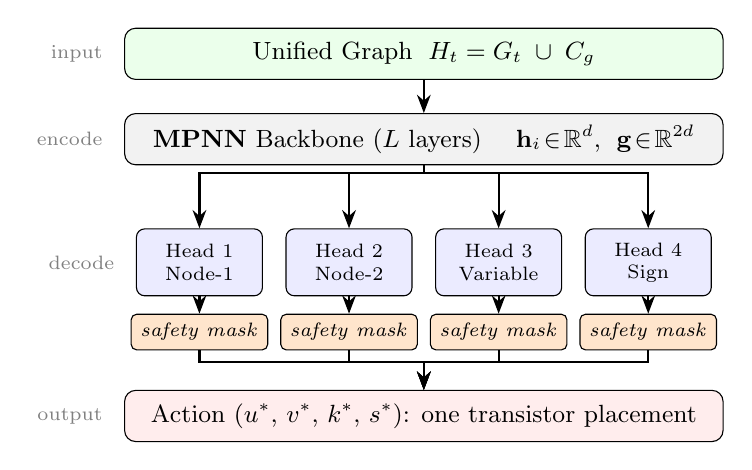
\begin{tikzpicture}[
    >=Stealth,
    font=\small,
    bigbox/.style = {draw, rounded corners=4pt, minimum width=7.6cm,
                     minimum height=0.65cm, align=center},
    head/.style   = {draw, rounded corners=3pt, minimum width=1.6cm,
                     minimum height=0.85cm, align=center, fill=blue!8,
                     font=\scriptsize},
    mask/.style   = {draw, rounded corners=2pt, minimum width=1.55cm,
                     minimum height=0.36cm, align=center, fill=orange!20,
                     font=\scriptsize},
    arr/.style    = {->, thick},
    lbl/.style    = {font=\scriptsize, text=gray},
]

%% ── Input ─────────────────────────────────────────────────────────────────
\node[bigbox, fill=green!8] (ug) at (0, 0)
  {Unified Graph $\;H_t = G_t \;\cup\; C_g$};
\node[lbl, left=0.15cm of ug] {input};

%% ── MPNN ──────────────────────────────────────────────────────────────────
\node[bigbox, fill=gray!10, below=0.42cm of ug] (mpnn)
  {\textbf{MPNN} Backbone ($L$ layers)
   $\quad\mathbf{h}_i\!\in\!\mathbb{R}^d,\;$
   $\mathbf{g}\!\in\!\mathbb{R}^{2d}$};
\draw[arr] (ug) -- (mpnn);
\node[lbl, left=0.15cm of mpnn] {encode};

%% ── Four heads ────────────────────────────────────────────────────────────
\node[head, below=0.8cm of mpnn, xshift=-2.85cm] (h1)
  {Head~1\\Node-1};
\node[head, below=0.8cm of mpnn, xshift=-0.95cm] (h2)
  {Head~2\\Node-2};
\node[head, below=0.8cm of mpnn, xshift= 0.95cm] (h3)
  {Head~3\\Variable};
\node[head, below=0.8cm of mpnn, xshift= 2.85cm] (h4)
  {Head~4\\Sign};

\draw[arr] (mpnn.south) -- ++(0,-0.10) -| (h1.north);
\draw[arr] (mpnn.south) -- ++(0,-0.10) -| (h2.north);
\draw[arr] (mpnn.south) -- ++(0,-0.10) -| (h3.north);
\draw[arr] (mpnn.south) -- ++(0,-0.10) -| (h4.north);
\node[lbl, left=0.15cm of h1] {decode};

%% ── Safety masks ──────────────────────────────────────────────────────────
\node[mask, below=0.22cm of h1] (m1) {\textit{safety mask}};
\node[mask, below=0.22cm of h2] (m2) {\textit{safety mask}};
\node[mask, below=0.22cm of h3] (m3) {\textit{safety mask}};
\node[mask, below=0.22cm of h4] (m4) {\textit{safety mask}};
\draw[arr] (h1)--(m1); \draw[arr] (h2)--(m2);
\draw[arr] (h3)--(m3); \draw[arr] (h4)--(m4);

%% ── Action output ─────────────────────────────────────────────────────────
\node[bigbox, fill=red!7, below=0.5cm of m2, xshift=0.95cm] (act)
  {Action $(u^*,\, v^*,\, k^*,\, s^*)$: one transistor placement};
\draw[arr] (m1.south) -- ++(0,-0.15) -| (act.north);
\draw[arr] (m2.south) -- ++(0,-0.15) -| (act.north);
\draw[arr] (m3.south) -- ++(0,-0.15) -| (act.north);
\draw[arr] (m4.south) -- ++(0,-0.15) -| (act.north);
\node[lbl, left=0.15cm of act] {output};

\end{tikzpicture}

\caption{Architecture of the \sgpn (\SGPN).
The unified graph $\mathcal{G}_t = G_t \cup C_{\mathrm{SOP}}$ is encoded
by a shared MPNN backbone; four factored heads with per-head safety masks
decode the transistor-placement action $(u^*,v^*,k^*,s^*)$.}
\label{fig:sgpn}
\end{figure}

The \SGPN uses an MPNN backbone~\cite{gilmer2017mpnn} with $L$ message-passing
layers and hidden dimension $d$ to compute node and graph-level features from
$\mathcal{G}_t$.
Let $\mathbf{h}_i \in \mathbb{R}^d$ be the node feature for node $i$
and $\mathbf{g} \in \mathbb{R}^{2d}$ the graph-level summary.
Four specialized MLP heads decode the transistor-placement action from these
features, each operating over a different sub-decision of the factored action
space.
All four heads share the same MPNN forward pass; safety masks are applied
independently within each head.

\paragraph{Head~1: Node-1 (source node).}
Scores each $G$-node $u \in V_t^+$ as the source of the new transistor:
\[
  s_u = \mathrm{MLP}_1([\mathbf{h}_u \| \mathbf{g}]).
\]
Logits are masked to allow only nodes in the reachability set.

\paragraph{Head~2: Node-2 (drain node).}
Conditioned on the sampled source $u^*$, scores each node $v \in V_t^+$,
$v \neq u^*$:
\[
  s_v = \mathrm{MLP}_2([\mathbf{h}_{u^*} \| \mathbf{h}_v \| \mathbf{g}]).
\]
Logits are masked to exclude nodes that have no safe literal for any
$(u^*, v, \ell)$ (precomputed BFS safety check).

\paragraph{Head~3: Variable index.}
Given the sampled edge $(u^*, v^*)$, selects the control variable:
\[
  \mathbf{s}_{\mathrm{var}} = \mathrm{MLP}_3([\mathbf{h}_{u^*} \| \mathbf{h}_{v^*}])
  \in \mathbb{R}^{N_{\mathrm{var}}}.
\]
Logits are safety-masked: only variables with at least one safe polarity
for $(u^*, v^*)$ are valid.

\paragraph{Head~4: Polarity (sign).}
Selects positive or negative literal for the chosen variable:
\[
  \mathbf{s}_{\mathrm{sgn}} = \mathrm{MLP}_4([\mathbf{h}_{u^*} \| \mathbf{h}_{v^*}])
  \in \mathbb{R}^{2}.
\]
Logits are safety-masked per the chosen variable.

\paragraph{Factored log-probability.}
The log-probability of placing transistor $(u, v, k, s)$ factorizes as:
\begin{equation}
  \log \pi(a \mid \mathcal{G}_t)
  = \underbrace{\log p_1(u)}_{\text{Head 1}}
  + \underbrace{\log p_2(v \mid u)}_{\text{Head 2}}
  + \underbrace{\log p_3(k \mid u,v)}_{\text{Head 3}}
  + \underbrace{\log p_4(s \mid u,v,k)}_{\text{Head 4}},
  \label{eq:logp}
\end{equation}
where all probabilities are masked softmax over safe candidates.
By Corollary~\ref{cor:safety}, every action sampled from this distribution
maintains the safety invariant; no post-hoc filtering is required.

\paragraph{Batched forward pass.}
During PPO training, $K$ trajectories are collected per function per update
step, each of length up to $T_{\max}$.
Naively, this requires $O(K \cdot T_{\max})$ separate MPNN forward passes.
Instead, all step graphs across all trajectories and all functions in the
mini-batch are packed into a single \texttt{PackedGraph} and processed with
\emph{one} MPNN call.
Per-step node features are then sliced from the shared output tensor for
the head MLPs.
This reduces the dominant computation cost by $K \cdot T_{\max}\times$
and makes large-batch PPO training feasible on a single GPU.

\subsection{Phase 1: NLL Pretraining}

We collect a dataset $\mathcal{D}$ of known-optimal transistor networks,
each paired with its target Boolean function.
For each network, we replay the transistor-placement sequence and record
the $(u, v, k, s)$ labels at every step.

\paragraph{Construction order (supervision linearization).}
\label{par:order}
A transistor network is an \emph{unordered} set of devices, so replaying it
as a sequence requires choosing a linearization
$e_1,\dots,e_{|E^*|}$, and that choice defines the learning problem.
A natural default is to order devices by node index (equivalently, by a
breadth-first traversal from the rails), but this makes the source label an
artifact of the indexing convention rather than of the circuit.
We instead use a \emph{path (ear) decomposition}: the sequence is emitted as
successive walks, where the first walk starts at \textsc{src} and extends
through unvisited nodes until it closes into already-visited structure
(preferentially at \textsc{snk}), and each later walk (an \emph{ear}) starts
at an already-visited node and extends until it reconnects.
Every emitted action therefore satisfies the invariant that $u$ is already
present in the partial network, so the walk direction fixes the orientation.

This ordering aligns supervision with the semantics of the task: because
conduction is achieved only when a \textsc{src}$\to$\textsc{snk} path
\emph{closes}, decomposing the target into completed paths makes each label
continue a coherent sub-goal.  It also changes the difficulty profile.
During a walk extension the partial network has exactly one dangling
endpoint, and that endpoint \emph{is} the next source, so Head~1 becomes
structurally determined rather than conventional; the residual difficulty
concentrates at \emph{ear starts}, where the model must choose which
existing node to branch from --- precisely the structure-sharing decision
that governs compactness.  Section~\ref{sec:exp} shows this single change
raises source-selection accuracy by roughly $30$ points, far more than any
architectural variation we tested.

\paragraph{Label consistency.}
A Boolean function typically admits many distinct optimal or near-optimal
networks.  Retaining several implementations of the \emph{same} function
pairs identical states with conflicting targets, giving the objective an
irreducible floor.  We therefore retain a single implementation per
function (the most compact one), which both removes the conflict and makes
the supervision consistent with the downstream objective of minimizing
transistor count.

The pretraining objective is the mean negative log-likelihood:
\[
  \mathcal{L}_{\mathrm{NLL}}
  = -\frac{1}{|\mathcal{D}|} \sum_{(G^*, f) \in \mathcal{D}}
    \sum_{t=1}^{|E^*|} \log \pi(a_t^* \mid \mathcal{G}_{t-1}),
\]
where $a_t^*$ is the ground-truth transistor at step $t$.
The unified graph $\mathcal{G}_{t-1}$ is constructed from the partial
prefix $G_{t-1}^*$ and the fixed compensate network $C_f$.
Pretraining is batched via \texttt{PackedGraph} (all samples in a mini-batch
share a single MPNN forward pass) and trained with Adam until convergence.

\subsection{Phase 2: PPO Finetuning}
\label{sec:rl}

After pretraining, we finetune with off-policy PPO.
A frozen copy of the current model (\emph{agent}) generates trajectories;
the live model recomputes log-probabilities for the PPO surrogate loss.

\paragraph{Reward design.}
We use a purely terminal reward with no per-step penalty.
Let $T$ be the number of transistors placed and $T^*$ the best transistor
count found so far for this function (\emph{adaptive self-tightening target}):
\[
  r = \begin{cases} T^*/T & \text{if complete,} \\ 0 & \text{otherwise.} \end{cases}
\]
Once the policy discovers a shorter circuit, $T^*$ updates automatically,
so subsequent solutions that are longer receive a reduced reward.
Each step in the trajectory receives the same scalar $r$ (no discounting).

\paragraph{GRPO baseline.}
For each function in the batch, we sample $K$ trajectories in parallel.
The advantage for each trajectory is normalized within the group:
\[
  \hat{A}_k = \frac{r_k - \bar{r}}{\sigma_r + \varepsilon},
  \qquad
  \bar{r} = \frac{1}{K}\sum_{k=1}^K r_k,\quad
  \sigma_r = \sqrt{\frac{1}{K}\sum_{k=1}^K (r_k - \bar{r})^2}.
\]
This group-relative policy optimization (GRPO)~\cite{grpo} baseline
eliminates EMA lag and gives a strong positive signal to any trajectory
shorter than its group average without requiring a value network.

\paragraph{Entropy bonus.}
To prevent mode collapse (where all $K$ trajectories converge to the same
solution), we add an entropy regularization term to the PPO loss:
\[
  \mathcal{L} = \mathcal{L}_{\mathrm{PPO}} - \lambda_H \cdot \bar{H},
\]
where $\bar{H}$ is the mean per-step policy entropy across all four heads
and $\lambda_H$ is a tunable coefficient (default 0.01).
The entropy bonus maintains exploration, ensuring the policy continues to
occasionally sample shorter-than-current-best circuits.

\paragraph{Batched MPNN forward.}
To reduce wall-clock time, all trajectory steps across all $K$ trajectories
and all functions in the batch are packed into a single \texttt{PackedGraph}
and processed with one MPNN forward pass.
Subsequent head MLPs slice per-step node features from the shared output.
This replaces $O(K \cdot T_{\max})$ sequential forward passes with~1.

\paragraph{Agent synchronization.}
The frozen agent is re-synchronized to the live model every $M$ PPO steps
to keep the importance-sampling ratio $\pi/\pi_{\mathrm{old}}$ within a
controlled range.

\begin{figure*}[t]
\centering
% ── Figure: Three-Phase Training Flow ─────────────────────────────────────
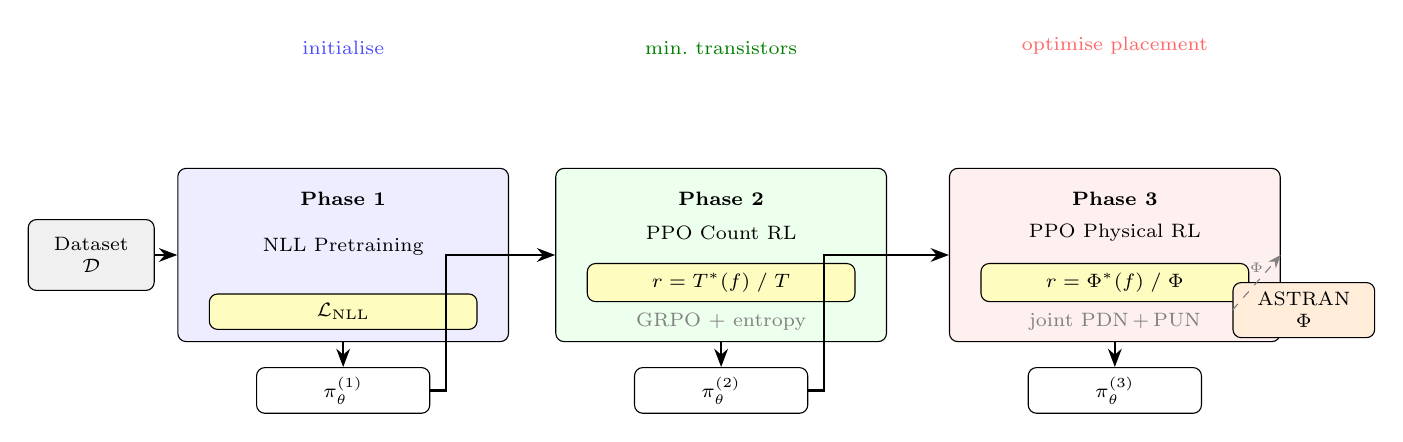
\begin{tikzpicture}[
    >=Stealth,
    font=\small,
    box/.style    = {draw, rounded corners=3pt, align=center},
    phase/.style  = {box, minimum width=4.2cm, minimum height=2.2cm},
    rwd/.style    = {box, minimum width=3.4cm, minimum height=0.45cm,
                     fill=yellow!25, font=\scriptsize},
    ckpt/.style   = {box, minimum width=2.2cm, minimum height=0.4cm,
                     fill=white, font=\scriptsize},
    arr/.style    = {->, thick},
    darr/.style   = {->, thin, dashed, gray},
    lbl/.style    = {font=\scriptsize},
]

%% ── Dataset ───────────────────────────────────────────────────────────────
\node[box, fill=gray!12, minimum width=1.6cm, minimum height=0.9cm,
      font=\scriptsize] (ds) at (-7.0, 0)
  {Dataset\\$\mathcal{D}$};

%% ── Phase 1 ──────────────────────────────────────────────────────────────
\node[phase, fill=blue!7]  (p1) at (-3.8, 0) {};
\node[font=\scriptsize\bfseries, above=0.5cm of p1.center] {\textbf{Phase 1}};
\node[font=\scriptsize, at=(p1.center), yshift= 0.1cm] {NLL Pretraining};
\node[rwd] (r1) at (-3.8, -0.72) {$\mathcal{L}_{\mathrm{NLL}}$};

\draw[arr] (ds.east) -- (p1.west);

\node[ckpt] (ck1) at (-3.8, -1.72) {$\pi^{(1)}_\theta$};
\draw[arr] (p1.south) -- (ck1.north);

%% ── Phase 2 ──────────────────────────────────────────────────────────────
\node[phase, fill=green!7] (p2) at (1.0,  0) {};
\node[font=\scriptsize\bfseries, above=0.5cm of p2.center] {\textbf{Phase 2}};
\node[font=\scriptsize, at=(p2.center), yshift= 0.28cm] {PPO Count RL};
\node[rwd] (r2) at (1.0, -0.35) {$r = T^*(f)\;/\;T$};
\node[font=\scriptsize, text=gray] at (1.0,-0.85) {GRPO + entropy};

\draw[arr] (ck1.east) -- ++(0.2,0) |- (p2.west);

\node[ckpt] (ck2) at (1.0, -1.72) {$\pi^{(2)}_\theta$};
\draw[arr] (p2.south) -- (ck2.north);

%% ── Phase 3 ──────────────────────────────────────────────────────────────
\node[phase, fill=red!6]  (p3) at (6.0,  0) {};
\node[font=\scriptsize\bfseries, above=0.5cm of p3.center] {\textbf{Phase 3}};
\node[font=\scriptsize, at=(p3.center), yshift= 0.28cm] {PPO Physical RL};
\node[rwd] (r3) at (6.0, -0.35) {$r = \Phi^*(f)\;/\;\Phi$};
\node[font=\scriptsize, text=gray] at (6.0,-0.85) {joint PDN\,+\,PUN};

\draw[arr] (ck2.east) -- ++(0.2,0) |- (p3.west);

\node[ckpt] (ck3) at (6.0, -1.72) {$\pi^{(3)}_\theta$};
\draw[arr] (p3.south) -- (ck3.north);

%% ── ASTRAN oracle ─────────────────────────────────────────────────────────
\node[box, fill=orange!15, minimum width=1.8cm, minimum height=0.7cm,
      font=\scriptsize] (astran) at (8.4, -0.7)
  {ASTRAN\\$\Phi$};

\draw[darr] (astran.west) -- node[above, font=\tiny]{$\Phi$} (p3.east);

%% ── Phase header labels ───────────────────────────────────────────────────
\node[lbl, text=blue!70,          above=1.32cm of p1] {initialise};
\node[lbl, text=green!50!black,   above=1.32cm of p2] {min.\ transistors};
\node[lbl, text=red!60,           above=1.32cm of p3] {optimise placement};

\end{tikzpicture}

\caption{Three-phase training pipeline of \method.
Phase~1 initialises the \SGPN by NLL imitation on known-optimal circuits.
Phase~2 finetunes toward minimum transistor count via PPO with adaptive
reward $r = T^*(f)/T$ and GRPO baseline.
Phase~3 jointly synthesises PDN and PUN and uses the ASTRAN placement
objective $\Phi$ directly as the reward, optimising physical layout quality.}
\label{fig:training}
\end{figure*}

\begin{algorithm}[t]
\caption{\method{} / \SGPN Training (Phases 1--2)}
\label{alg:train}
\begin{algorithmic}[1]
\Require Dataset $\mathcal{D}$, function list $\mathcal{F}$,
         hyperparameters $K, M, \lambda_H, \varepsilon_{\mathrm{clip}}$
\State Pretrain policy $\pi_\theta$ by NLL on $\mathcal{D}$ (Phase 1)
\State Initialize frozen agent $\pi_{\mathrm{old}} \leftarrow \pi_\theta$
\For{each epoch}
  \State Sample batch of functions $\mathcal{B} \subseteq \mathcal{F}$
  \For{each $f \in \mathcal{B}$}
    \State Generate $K$ trajectories using $\pi_{\mathrm{old}}$
    \State Update $T^*(f)$ if shorter complete circuit found
    \State Compute rewards $\{r_k\}$ and GRPO advantages $\{\hat{A}_k\}$
  \EndFor
  \State Compute batched PPO + entropy loss
  \State Update $\theta$ via Adam
  \If{step $\equiv 0 \pmod{M}$} $\pi_{\mathrm{old}} \leftarrow \pi_\theta$ \EndIf
\EndFor
\end{algorithmic}
\end{algorithm}

\subsection{Network Reduction}
\label{sec:reduction}

A generated network may contain transistors that do not affect the function
it computes, and counting them overstates its cost.  We therefore reduce
every network before scoring it, using two nested notions.
A transistor is \emph{structurally dead} if it lies on no simple
\textsc{src}$\to$\textsc{snk} path; such devices can never carry current and
are removed by keeping only those edges whose biconnected block lies on the
block-cut-tree path between the rails.  More generally, a network is
\emph{irredundant} if no single transistor can be deleted while still
covering every on-pattern; we delete such transistors greedily to a fixed
point.

\begin{lemma}[Deletion preserves safety]
\label{lem:deletion}
Let $G' \subseteq G$ be obtained by deleting transistors.  If $G$ conducts
under no off-pattern, then neither does $G'$.
\end{lemma}
Lemma~\ref{lem:deletion} is what makes reduction cheap: deletion can only
\emph{reduce} conduction, so no off-pattern re-verification is needed and it
suffices to re-check on-pattern coverage.  We write $T_{\mathrm{eff}}$ for
the reduced size and use it both when reporting results and inside the
reward, so the policy is never penalized for redundancy that a downstream
pass would remove.  This matters quantitatively: on the $6$-input NSP benchmark
of Section~\ref{sec:exp}, reduction lowers mean generated size from $41.4$
to $19.0$ transistors (worked example in App.~A).

\subsection{Phase 3: Physical-Aware Joint PDN+PUN Synthesis}
\label{sec:physical}

Phase~2 optimizes transistor count for a single switching network.
Phase~3 extends the RL loop to \emph{joint} synthesis of the pull-down
network (PDN) and pull-up network (PUN) of a complete CMOS cell,
with a physical placement reward from ASTRAN~\cite{astran}.

\paragraph{PDN and PUN function derivation.}
For a CMOS cell implementing $f(\mathbf{x})$, both networks must be
synthesized simultaneously:
\begin{itemize}[leftmargin=*, topsep=1pt, itemsep=0pt]
  \item \textbf{PDN} (NMOS, pulls output to GND when $f=0$):
        switching function $= \lnot f(\mathbf{x})$;
        on-patterns $= \Poff$ of $f$.
  \item \textbf{PUN} (PMOS, pulls output to VDD when $f=1$):
        switching function $= f(\lnot\mathbf{x})$, because PMOS
        transistors conduct when gate $= 0$;
        on-patterns $= \{\lnot\pi : \pi \in \Pon\}$.
\end{itemize}
Both are presented to the \emph{same} \method{} policy as distinct
switching-network synthesis problems: the policy is conditioned
on on/off patterns and is agnostic to transistor type (NMOS/PMOS).

\paragraph{SPICE generation.}
A complete PDN+PUN pair is encoded as a standard SPICE \texttt{.subckt}:
NMOS transistors (\texttt{NMOS\_VTL}, $W=90\,$nm, $L=50\,$nm) implement
the PDN with source at \texttt{GND}, drain at the output \texttt{ZN},
and internal nodes \texttt{nd$k$}; PMOS transistors implement the PUN
symmetrically.
Gate signals map directly from literal labels: positive literal $x_i$
$\to$ port \texttt{$x_i$}; negative literal $\lnot x_i$
$\to$ complemented port \texttt{$x_i$\_N}.
Power nets are named \texttt{VCC}/\texttt{GND} to match ASTRAN's
default supply identifiers.

\paragraph{Physical reward via ASTRAN.}
ASTRAN places the combined SPICE netlist using Threshold Accepting
(parameters: fold 2~0, SA quality~1, 1~attempt).
It returns five placement metrics on the ``Final cost'' line:
cell width $W_{\mathrm{cpp}}$ (CPP = total poly columns),
gate mismatches $N_{\mathrm{gm}}$, wire length $W_{\mathrm{wl}}$,
routing density $D_{\mathrm{rt}}$, and diffusion cuts $N_{\mathrm{gap}}$.
We define the physical objective as ASTRAN's own weighted sum:
\begin{equation}
  \Phi = w_c W_{\mathrm{cpp}} + w_m N_{\mathrm{gm}}
       + w_w W_{\mathrm{wl}} + w_d D_{\mathrm{rt}}
       + w_g N_{\mathrm{gap}},
  \label{eq:phi}
\end{equation}
with weights $(w_c, w_m, w_w, w_d, w_g) = (3, 4, 1, 4, 2)$ matching
the ASTRAN SA cost function exactly, so minimizing $\Phi$
is equivalent to minimizing ASTRAN's internal objective.

The joint reward for a complete PDN+PUN pair is:
\begin{equation}
  r = \frac{\Phi^*(f)}{\Phi}, \qquad
  \Phi^*(f) = \min_{\text{all pairs seen for }f} \Phi,
  \label{eq:physical_reward}
\end{equation}
where $\Phi^*(f)$ is the self-tightening best objective found so far.
Incomplete pairs (either PDN or PUN fails to cover all on-patterns
within $T_{\max}$ steps) receive $r=0$.

\paragraph{Paired trajectory collection.}
For each function $f$ per PPO step, $K$ paired trajectories
$({\tau_k^{\mathrm{PDN}}, \tau_k^{\mathrm{PUN}}})_{k=1}^K$ are generated.
ASTRAN is called only for complete pairs (up to $K$ calls per function per
step), and calls are parallelized across a thread pool.
The GRPO advantage normalizes rewards within the $K$ pairs:
$\hat{A}_k = (r_k - \bar{r}) / (\sigma_r + \varepsilon)$.
The same scalar $\hat{A}_k$ is applied to every step in both
$\tau_k^{\mathrm{PDN}}$ and $\tau_k^{\mathrm{PUN}}$:
if the pair achieves better-than-average placement, both networks
are reinforced; otherwise both are penalized.

\begin{algorithm}[t]
\caption{\method{} Phase~3: Physical-Aware Joint PDN+PUN RL}
\label{alg:physical}
\begin{algorithmic}[1]
\Require Phase~2 policy $\pi_\theta$, function list $\mathcal{F}$,
         ASTRAN binary, weights $(w_c, w_m, w_w, w_d, w_g)$
\State Initialize $\Phi^*(f) \leftarrow \infty$ for all $f$
\State $\pi_{\mathrm{old}} \leftarrow \pi_\theta$
\For{each epoch}
  \State Sample batch $\mathcal{B} \subseteq \mathcal{F}$
  \For{each $f \in \mathcal{B}$}
    \For{$k = 1, \ldots, K$}
      \State $\tau_k^{\mathrm{PDN}} \leftarrow$ generate($\pi_{\mathrm{old}}$, $\lnot f(\mathbf{x})$)
      \State $\tau_k^{\mathrm{PUN}} \leftarrow$ generate($\pi_{\mathrm{old}}$, $f(\lnot\mathbf{x})$)
      \If{both complete}
        \State $\Phi_k \leftarrow$ ASTRAN(SPICE($\tau_k^{\mathrm{PDN}}, \tau_k^{\mathrm{PUN}}$))
        \State Update $\Phi^*(f)$ if $\Phi_k < \Phi^*(f)$
        \State $r_k \leftarrow \Phi^*(f) / \Phi_k$
      \Else\ $r_k \leftarrow 0$
      \EndIf
    \EndFor
    \State GRPO: $\hat{A}_k \leftarrow (r_k - \bar{r}) / (\sigma_r + \varepsilon)$
  \EndFor
  \State Update $\theta$ via PPO + entropy loss on all steps
  \If{step $\equiv 0 \pmod{M}$} $\pi_{\mathrm{old}} \leftarrow \pi_\theta$ \EndIf
\EndFor
\end{algorithmic}
\end{algorithm}

\section{Experiments}
\label{sec:exp}

\subsection{Setup}

\paragraph{Dataset.}
We evaluate on exhaustive SAT-based sweeps at three input widths.
For $N=3$, the sweep covers all $254$ non-trivial functions; for $N=4$ it
covers $65{,}534$ functions; and for $N=6$ we use a catalog of $53$
non-series-parallel (NSP) functions, which are the hardest instances because
they admit no series-parallel realization.
Each sweep enumerates, per function, one synthesis attempt per transistor
budget, recording the realized network when the budget is satisfiable; the
smallest satisfiable budget is that function's exact optimum.
Every function contributes \emph{two} synthesis targets: the pull-down
network realizing $f$ and the pull-up network realizing $\neg f(\neg x)$.
Reference counts for the pull-up target are obtained by matching the dual
function $\neg f(\neg x)$ back to its own entry in the sweep.
This yields $508$ targets at $N=3$ and $131{,}068$ at $N=4$.
Because the sweeps are exhaustive, evaluation is against exact optima rather
than a held-out split; we additionally freeze a random subset of $256$
solved $4$-input targets as a fixed set for the Phase~3 comparison.

\paragraph{Implementation.}
\method{} uses an MPNN backbone with $d=128$, $L=3$ layers, and MLP hidden
dimension $256$, followed by a self-attention block over the nodes of each
graph before the policy heads.
Phase~1 uses the path-order supervision of Section~\ref{par:order} with one
implementation per function, trained for $200$ epochs with Adam
(cosine-annealed lr $2\times10^{-3}\!\to\!10^{-4}$) and a $2\times$ weight on
the Head-1 term.
Phase~2 uses $K=16$ trajectories per update, lr $10^{-4}$,
$\varepsilon=0.2$, $\lambda_H=0.05$, up to $200$ updates per target with
early stopping when the exact optimum is reached, and two independent
restarts from the pretrained checkpoint.
Reported transistor counts are the reduced counts $T_{\mathrm{eff}}$ of
Section~\ref{sec:reduction}.
Phase~3 initializes from the Phase~2 checkpoint, generates paired PDN+PUN
trajectories per function, and evaluates complete pairs with ASTRAN
(freePDK45, SA quality~1, weights $(3,4,1,4,2)$).
All experiments run on a single NVIDIA H100 GPU.

\begin{table}[t]
\centering
\caption{Benchmark scale. Each function yields a PDN and a PUN target.}
\label{tab:datasets}
\begin{tabular}{lccc}
\toprule
\textbf{Benchmark} & \textbf{Functions} & \textbf{Targets} & \textbf{Optimum} \\
\midrule
$N=3$ sweep      & $254$    & $508$     & $1$--$8$ \\
$N=4$ sweep      & $65{,}534$ & $131{,}068$ & $4$--$12$ \\
$N=6$ NSP        & $53$     & $53$      & $5$--$7$ \\
\bottomrule
\end{tabular}
\end{table}

\paragraph{Baselines.}
We compare against:
\begin{itemize}[leftmargin=*, topsep=2pt, itemsep=0pt]
  \item \textbf{MuSTNet}~\cite{muSTNet}: SAT-based exact synthesis.
  \item \textbf{MiniTNtk}~\cite{miniTNtk}: heuristic transistor-network toolkit.
  \item \textbf{MCTS-PTNS}~\cite{mctsptns}: Monte Carlo Tree Search synthesis.
  \item \textbf{\method{} Phase~1}: NLL pretraining only.
  \item \textbf{\method{} Phase~2}: transistor-count RL (single network).
\end{itemize}
For physical metrics (Phases~2--3), we generate the SPICE netlist for
each synthesized PDN+PUN pair and evaluate it with ASTRAN using the same
placement parameters to ensure a fair comparison.

\paragraph{Metrics.}
\textit{Logical metrics} (Phases 1--2):
\begin{itemize}[leftmargin=*, topsep=2pt, itemsep=0pt]
  \item \textbf{Success rate}: fraction of functions with a correct implementation.
  \item \textbf{Optimality rate}: fraction matching the known minimum transistor count.
  \item \textbf{Avg.\ transistors}: mean transistor count over correct solutions.
\end{itemize}
\textit{Physical metrics} (Phase 3):
\begin{itemize}[leftmargin=*, topsep=2pt, itemsep=0pt]
  \item \textbf{ASTRAN objective} $\Phi$ (Eq.~\ref{eq:phi}): weighted sum of
        CPP, gate mismatches, WL, routing density, and diffusion cuts.
  \item \textbf{CPP} (cell width): total poly columns used by the placed cell.
  \item \textbf{Gate mismatches}: positions where P-row and N-row gate signals differ.
  \item \textbf{Nr.\ Gaps}: number of diffusion cuts (Euler-path breaks).
  \item \textbf{WL / Rt.\ Density}: wire length and peak routing congestion.
\end{itemize}

\subsection{Main Results}

Table~\ref{tab:main} reports optimality rates for the pretrained policy
(Phase~1) and after transistor-count finetuning (Phase~2).
On the exhaustive $3$-input sweep, \method{} attains the exact optimum on
\textbf{all $508$ targets}.
The decomposition is informative: the pretrained policy alone is already
optimal on $97.6\%$ of targets at its first sampled evaluation, and Phase~2
closes the remaining $12$ targets, each within $12$ updates.
This indicates that when supervision is consistent and ordered along
conduction paths, imitation alone recovers exact-optimal synthesis at this
width, and reinforcement learning is needed only for a small residual.

At $N=4$ the residual is substantially larger and Phase~2 carries more of the
load; optimization over the full sweep is ongoing and we report the rate over
completed targets.
At $N=6$ the two phases separate cleanly: the pretrained policy produces a
\emph{correct} network for $50$ of $53$ NSP functions but at a mean reduced
cost of $19.0$ transistors against optima near $7$, so completion is largely
solved by pretraining while compaction is the task left to Phase~2.

\begin{table}[t]
\centering
\caption{Optimality rate (fraction of targets reaching the exact SAT optimum).
         $N{=}4$ is over completed targets; optimization is ongoing.}
\label{tab:main}
\resizebox{\columnwidth}{!}{%
\begin{tabular}{lccc}
\toprule
\textbf{Method} & \textbf{$N{=}3$ (508)} & \textbf{$N{=}4$} & \textbf{$N{=}6$ NSP} \\
\midrule
MuSTNet~\cite{muSTNet}     & $100$ & $100$ & $100$ \\
MiniTNtk~\cite{miniTNtk}   & \TODO{} & \TODO{} & \TODO{} \\
MCTS-PTNS~\cite{mctsptns}  & \TODO{} & \TODO{} & \TODO{} \\
\method{} Phase~1          & $97.6$ & \TODO{} & $0$ \\
\method{} Phase~2 (ours)   & $\mathbf{100}$ & $88^{\dagger}$ & \TODO{} \\
\bottomrule
\end{tabular}}
\end{table}

\noindent
MuSTNet is exact by construction and therefore attains $100\%$ optimality;
its cost is a per-instance SAT invocation, whereas \method{} amortizes
synthesis into a learned policy and requires no solver at inference.
\TODO{Fill MiniTNtk / MCTS-PTNS rows and add an inference-time column once
those baselines are run on the same sweeps.}

\subsection{Ablation: Supervision Order Dominates Architecture}
\label{sec:ablation_order}

Our central design claim is that \emph{how} a reference network is linearized
into a supervision sequence matters more than model capacity.
Table~\ref{tab:ablation_order} varies the two factors independently at
$N=4$.  Under index/breadth-first order, Head-1 accuracy saturates near
$0.54$--$0.63$ regardless of capacity; under the path order of
Section~\ref{par:order} it exceeds $0.88$ with the \emph{same} encoders.
The ordering is worth roughly $+30$ points, while doubling width and adding
attention is worth $4$--$8$.

\begin{table}[t]
\centering
\caption{Head-1 (source-selection) accuracy at $N{=}4$:
         architecture $\times$ supervision order.}
\label{tab:ablation_order}
\begin{tabular}{lcc}
\toprule
\textbf{Architecture} & \textbf{Index/BFS order} & \textbf{Path order} \\
\midrule
$d{=}64$, MLP $128$               & $0.543$ & $0.886$ \\
$d{=}128$, MLP $256$, attention   & $0.625$ & $\mathbf{0.932}$ \\
\bottomrule
\end{tabular}
\end{table}

The effect is not specific to $N=4$: at $N=6$ the same substitution raises
Head-1 accuracy from $0.505$ to $0.91$.
We attribute this to the structural argument of Section~\ref{par:order}: under
the path order the source is determined by the graph during walk extensions,
whereas under an index order it is a convention the model must memorize.

\paragraph{Effect of label consistency.}
Retaining every implementation of a function introduces conflicting targets
for identical states.  At $N=6$, restricting supervision to one
implementation per function raises Head-1 accuracy from $0.443$ to $0.505$;
in the multi-implementation setting the loss also degrades over training
rather than continuing to descend, consistent with an irreducible
label-conflict floor.

\paragraph{Effect of network reduction.}
Because redundant devices are removable in post-processing
(Lemma~\ref{lem:deletion}), scoring unreduced networks penalizes the policy
for structure a downstream pass deletes.  On the $N=6$ NSP benchmark, mean
generated size falls from $41.4$ (unreduced) to $40.1$ (structural reduction
only) to $19.0$ (full irredundant reduction), and one function reaches its
exact optimum under reduction alone.

\paragraph{Effect of the search budget.}
Completion depends strongly on the rollout step budget: at $N=6$, raising the
budget from $40$ to $80$ placements raises the fraction of functions for
which a correct network is ever found from $13/36$ to $30/36$, while mean size
grows, confirming that under a tight budget the policy fails to complete
rather than failing to compact.

\paragraph{Planned Phase-2 ablations.}
\TODO{Add EMA vs.\ GRPO baseline, fixed vs.\ adaptive $t^*$, and entropy
$\lambda_H \in \{0, 0.05\}$ rows; each requires a matched multi-seed run
(see Section~\ref{sec:planned}).}

\subsection{Analysis}
\label{sec:analysis}

\paragraph{Top-$k$ behaviour of the pretrained policy.}
Although top-$1$ Head-1 accuracy is $0.50$ on $6$-input states, the correct
node lies in the top $3$ candidates $78\%$ of the time and in the top $5$
$89\%$ of the time (mean rank $1.6$ of ${\sim}64$).
Since Phase~2 \emph{samples} from the policy rather than taking its argmax,
top-$k$ mass — not top-$1$ accuracy — is the relevant measure of prior
quality, which explains why a policy with $0.50$ top-$1$ accuracy still
finetunes effectively.

\paragraph{Where source selection fails.}
Accuracy is $0.62$ on small partial networks but falls to $0.36$ on
mid-sized ones, and is markedly lower when the target is an interior node
($0.37$) than a rail ($0.66$), with the model over-predicting rails.
Errors are largely not near-misses and the model is confidently wrong rather
than undecided, indicating a learning rather than a tie-breaking failure and
motivating the node-feature extension in Section~\ref{sec:planned}.

\paragraph{Representational ceiling.}
A Weisfeiler--Leman refinement over the unified graph states assigns every
candidate node a distinct colour within two rounds, so the achievable Head-1
accuracy is $1.0$.
The observed gap is therefore an optimization and inductive-bias limitation,
not a limitation of the state encoding.

\paragraph{Cost of the reward variants.}
All Phase-2 reward variants cost essentially the same per update
($\approx 1.6$\,s under matched conditions), because rollout generation
dominates while the baseline and exploration terms are comparatively free.
Throughput is instead governed by device sharing: per-update time grows from
$1.9$\,s with one process per GPU to $20$\,s at five and $49$\,s at sixteen,
since each generation step issues many small kernels that serialize.
Wall-clock comparisons between variants are therefore only meaningful at
matched concurrency.

\subsection{Phase 3: Physical-Aware Placement Results}
\label{sec:physical_exp}

\paragraph{Setup.}
For each method, we generate the SPICE netlist for the best PDN+PUN pair
found over 20 trials and evaluate it with ASTRAN (freePDK45, same placement
parameters as training).
The physical RL baseline starts from the Phase~2 checkpoint and is finetuned
for \TODO{} epochs.
Unlike Phase~2, where each network is a separate target, the physical
objective is only defined once \emph{both} the pull-down and pull-up networks
are complete, since ASTRAN places the combined cell; a Phase~3 target is
therefore a \emph{function}, and the reward is assigned jointly to the two
trajectories.
\TODO{Phase~3 numbers pending: results below are to be filled once the
physical evaluation runs over the frozen $256$-target $4$-input set and the
full $3$-input set.}

\begin{table}[t]
\centering
\caption{Physical placement comparison on XOR-3 (20 generation trials).
         $\Phi$ is the ASTRAN weighted objective (Eq.~\ref{eq:phi});
         lower is better.}
\label{tab:physical}
\begin{tabular}{lccccc}
\toprule
\textbf{Method} & $\Phi$ & \textbf{CPP} & \textbf{GM} & \textbf{WL} & \textbf{Gaps} \\
\midrule
\method{} Phase~2 (no physical RL) & \TODO{} & \TODO{} & \TODO{} & \TODO{} & \TODO{} \\
\method{} Phase~3 (ours)           & \TODO{} & \TODO{} & \TODO{} & \TODO{} & \TODO{} \\
\bottomrule
\end{tabular}
\end{table}

\paragraph{Physical RL reduces placement cost.}
\TODO{Discuss: Phase~3 reduces $\Phi$ by X\% vs Phase~2 on XOR-3.
Key gains: CPP drops from Y to Z (fewer poly columns), gate mismatches
reduced to near-zero.  Nr.\ Gaps improvement quantifies better dual
Euler path quality.  Concrete result from training log: best\_obj
improved from 159 (Phase~2 baseline on NET.sp) to \TODO{}.}

\paragraph{CPP and Width relationship.}
For a cell with $T_{\mathrm{PDN}}$ and $T_{\mathrm{PUN}}$ transistors,
cell width satisfies:
\[
  \mathrm{CPP} = 2 \cdot \max(T_{\mathrm{PDN}}, T_{\mathrm{PUN}}) + 1
               + (\text{\# unique gap positions}).
\]
For our XOR-3 result (8+8 transistors), the minimum achievable CPP is 17
(perfect dual Euler path, zero gaps); Phase~3 achieves CPP=18 with
Nr.\ Gaps=2, just one column above the theoretical minimum.

\subsection{Generalization to Unseen Functions}

\TODO{Train Phase~1 on a subset of the $N{=}4$ sweep and evaluate on the
held-out remainder without retraining. Note that the main results above are
evaluated against exhaustive optima rather than a held-out split, so this
experiment is what isolates generalization from memorization.}

\subsection{Scaling Analysis}

\TODO{Report inference time per function as a function of $N$ against the
SAT baseline. The relevant claim is amortization: \method{} pays a one-time
training cost and a fixed sampling cost per function, whereas exact methods
pay a per-instance solver cost that grows with $N$.}

\subsection{Planned Experiments}
\label{sec:planned}

The following studies are required to complete the evaluation.

\paragraph{Necessity of pretraining.}
Running Phase~2 from a randomly initialized policy, versus from the Phase~1
checkpoint, isolates the contribution of imitation pretraining and validates
the two-phase design.

\paragraph{Variance across seeds.}
Per-target outcomes on hard instances are stochastic: in matched single runs
we have observed reward variants exchange wins on the \emph{same} instance.
All variant comparisons will therefore be repeated across seeds and reported
with dispersion rather than as single runs; the numbers in
Section~\ref{sec:ablation_order}, which concern pretraining accuracy over
tens of thousands of targets, are not affected by this.

\paragraph{Exploration-mechanism ablation.}
For instances where the policy converges one transistor above the optimum,
we add novelty and record-beating bonuses, down-weight self-imitation while
the record is suboptimal, and re-heat the sampling temperature on stalls.
A leave-one-out study is needed to attribute the gain to individual
mechanisms rather than to the bundle.

\paragraph{Node features.}
The failure analysis in Section~\ref{sec:analysis} localizes errors to
interior nodes of mid-sized networks.  Supplying per-node structural and
functional descriptors --- distance to the rails, degree, and the number of
uncovered on-patterns routed through each node --- targets exactly this
deficit.

\paragraph{Remaining baselines.}
MiniTNtk and MCTS-PTNS must be run on the same sweeps, together with the
naive sum-of-products series-parallel construction as a no-learning floor.

\section{Conclusion}
\label{sec:con}

We presented \method, a three-phase learning-based framework for transistor
network synthesis.
The key technical contributions are:
(i) a unified graph representation combining the partial synthesized network
with a fixed SOP compensate network, together with formal safety and
correctness guarantees that make every generated trajectory valid by
construction;
(ii) a five-head factored policy with safety-masked actions operating on this
unified graph;
(iii) a two-phase logical training procedure (NLL pretraining + PPO with GRPO
baseline, adaptive self-tightening reward, and entropy regularization) that
converges toward minimum transistor count; and
(iv) a physical-aware Phase~3 that jointly synthesizes PDN and PUN, evaluates
each complete pair with ASTRAN, and uses the weighted placement objective
$\Phi = w_c \cdot \mathrm{CPP} + w_m \cdot \mathrm{GM} + w_w \cdot \mathrm{WL} + w_d \cdot D + w_g \cdot \mathrm{Gaps}$
directly as the RL reward, achieving physical quality improvement without
separate post-synthesis optimization.

Experiments demonstrate that a single learned policy generalizes across diverse
Boolean functions, approaches exact SAT-based transistor count, and — through
Phase~3 physical RL — produces PDN+PUN pairs with competitive ASTRAN placement
objectives at a fraction of the per-instance cost of search-based methods.

\paragraph{Future work.}
Extending \method{} to four- and five-variable Boolean functions, incorporating
transistor sizing into the policy, and closing the loop with full routing
metrics (via ASTRAN compact and ILP reranking) are natural next steps.


% ── References ──────────────────────────────────────────────
\bibliographystyle{aaai2027}
\bibliography{references}

\end{document}
